\documentclass[letterpaper, 11pt]{extarticle}

\usepackage[english]{babel}
\usepackage[margin = 1in]{geometry}

\usepackage{hyperref}

\usepackage{enumerate}
\usepackage[shortlabels]{enumitem}
\usepackage{framed}
\usepackage{csquotes}


\usepackage{float}
\usepackage{tabularx}
\usepackage{xcolor}
\usepackage{multicol}
\usepackage{subcaption}
\usepackage{caption}
\captionsetup{format = hang, margin = 10pt, font = small, labelfont = bf}

% Citation
\usepackage[round, authoryear]{natbib}

\usepackage{todonotes}
\usepackage{placeins}

% Hyperlinks setup
\usepackage{hyperref}
\definecolor{links}{rgb}{0.36,0.54,0.66}
\hypersetup{
   colorlinks = true,
    linkcolor = black,
     urlcolor = blue,
    citecolor = blue,
    filecolor = blue,
    pdfauthor = {Author},
     pdftitle = {Title},
   pdfsubject = {subject},
  pdfkeywords = {one, two},
  pdfproducer = {LaTeX},
   pdfcreator = {pdfLaTeX},
   }
   
\usepackage{titlesec}
\usepackage[many]{tcolorbox}

% Adjust spacing after the chapter title
\titlespacing*{\chapter}{0cm}{-2.0cm}{0.50cm}
\titlespacing*{\section}{0cm}{0.50cm}{0.25cm}

% Indent 
\setlength{\parindent}{0pt}
\setlength{\parskip}{1ex}
\usepackage{multirow}
\tcbset{
  disclaimerbox/.style={
    colback=yellow!20,    % Background color (light yellow)
    colframe=cyan!80!black, % Border color
    fonttitle=\bfseries,
    coltitle=white,
    boxrule=1.2pt,
    arc=4pt,
    left=4pt,
    right=4pt,
    top=4pt,
    bottom=4pt
  }
}
\begin{document}

\begin{Large}
    \textsf{\textbf{RoboCup Smart Manufacturing League: an Opinion Regarding the Future of RoboCup Industrial}}

RoboCup German Open Workshop Paper

\end{Large}

\vspace{1ex}
Tarik Viehmann, Matteo Tschesche, Wataru Uemura and Alexander Ferrein

\text{Version 1.0}

\text{4nd Feb 2026}


% \section*{Disclaimer}

\section{Introduction}
\begin{tcolorbox}[disclaimerbox, title=Disclaimer]
This document is a \textbf{concept draft} and \textbf{does not represent any official position} on the direction of the RoboCup Smart Manufacturing League.  
\textbf{It reflects the opinions of the authors} and is intended to present a coherent vision for the future, serving as a baseline for discussion.  

This document is partially derived from the document \emph{Embodied Autonomous Intelligence for On-Demand
Manufacturing: A RoboCup Industrial Workshop Proposal} (\url{ https://github.com/robocup-at-work/sml-embodied-autonomous-intelligence}), which we henceforth call the \emph{reference proposal}. Parts that share fundamental similarity are indicated using disclaimer boxes like this one. 


Feedback, questions, and constructive criticism are welcome. Please contact the authors directly or submit issues or pull requests via the associated GitHub repository:  
\url{https://github.com/robocup-sml/workshop-paper}
\end{tcolorbox}

% {\color{gray}
% The RoboCup Smart Manufacturing League (SML) \cite{dissanayaka2025productionlogisticssmartmanufacturing} is Robo\-Cup's new industrial competition format.
% From 2026 it will replace the existing Logistics and @Work leagues, presenting a major conceptual overhaul and future-proof long-term vision.

% The new concept aims to translate the knowledge and research advances from the former leagues
% into a novel robotic vision for modern production facilities.
% The goal is to create a flexible and fully autonomous 
% factory environment that shifts from traditional mass production — where goods are manufactured in large quantities and stored for long periods — to on-demand manufacturing. By enabling robots to autonomously produce and recycle products as needed, the league promotes a more sustainable and resource-efficient approach.
% Covering popular research areas, such as robotic intra-logistics, advanced object manipulation, and multi-robot plan optimization, the league aims to translate industry challenges into an exciting research, benchmarking, and competition format.
% }
The RoboCup Smart Manufacturing League (SML) \cite{dissanayaka2025productionlogisticssmartmanufacturing} is RoboCup's new industrial competition format, introduced in 2026 to expand on the legacy of the existing Logistics League and @Work League.
This transition represents a major conceptual overhaul, aiming to consolidate lessons learned from the former leagues while providing a long-term, future-proof vision for autonomous industrial robotics research.
This document presents a vision for the league that can inform and structure the creation of an official rulebook.

The motivation for creating SML stems from the evolving needs of modern production environments.
Traditional mass-production factories focus on high-volume manufacturing with extensive storage, but contemporary industrial challenges demand flexibility, on-demand production, and sustainability.
Both former leagues addressed essential yet largely isolated aspects of industrial robotics. The @Work League concentrated on precise object manipulation and mobile manipulation skills, advancing the core capabilities of industrial robots.
In contrast, the Logistics League focused on multi-robot coordination, autonomous intra-logistics, and workflow optimization under uncertainty at the system level.
While both leagues advanced their respective domains, neither modeled a complete factory scenario encompassing integrated production planning, on-demand manufacturing, warehouse management, and recycling processes; in particular, assembly processes, quality control, and human–robot interaction remained underrepresented.

The Smart Manufacturing League is designed to close this gap by integrating these previously isolated aspects into a coherent smart factory setting. Rather than addressing manipulation, logistics, or planning in isolation, the SML combines them within a unified framework that reflects the interdependencies of real-world production systems.
To guide this integration and ensure accessibility, relevance, and long-term impact, the league is structured around four core pillars:

\paragraph{1. Beginner friendliness through progressive difficulty}
The league lowers the entry barrier by introducing tasks with increasing levels of complexity, allowing teams to incrementally build up capabilities. Early stages focus on well-defined subtasks, while advanced scenarios introduce uncertainty, partial observability, and tighter integration of perception, planning, and execution.

\paragraph{2. Relevance for state-of-the-art research and future industrial applications}
The league provides standardized benchmarks that address open research problems in autonomous manufacturing, such as robust manipulation under uncertainty, dynamic task and motion planning, effective and safe human-robot collaboration and adaptive production scheduling.

\paragraph{3. Systematic exploration of specialization and generalization}
Specialization is enabled through dedicated competition tracks targeting individual functional areas of a smart factory, including intra-logistics, packaging and palletizing, and assembly tasks at workbenches.
These tracks follow the industrial trend of developing highly optimized solutions.
Generalization is fostered by also offering a unified factory challenge in which robots are rewarded for successfully performing a diverse set of tasks drawn from the specialized tracks and beyond.

\paragraph{4. Data-driven insights and benchmarking}
Standardized communication interfaces and data formats ensure that all interactions with the shared shop-floor environment are logged and accessible.
By aligning with established industrial standards, the league ensures that collected data is relevant, interoperable, and structured for reproducible evaluation.

Beyond its immediate competition format, the Smart Manufacturing League is designed to address unsolved problems that are expected to become central in future smart manufacturing scenarios. The league deliberately targets capabilities that remain underexplored or infeasible at current industrial scale, including robust manipulation under uncertainty, inspection and quality control, safe human–robot interaction and collaboration, as well as integrated dynamic planning and optimization. Industrial partners are consulted to ensure relevance, while challenges are formulated in an abstracted and affordable setting that enables systematic benchmarking and reproducible evaluation without the complexity and cost of full industrial deployment.

This paper presents the design principles, challenges, and goals of the SML, highlighting how it sets a new standard for robotic competitions in industrial settings.


% \section{Long-Term Vision}
% The long-term vision is to advance robotics research towards \emph{unsolved problems relevant for future
% smart manufacturing scenarios}.
% %
% The competition focuses on challenging robotic capabilities that
% remain underexplored or infeasible at current industrial scale. Industrial partners are consulted to
% shape industry-relevant challenges, while maintaining an abstracted and affordable experimental
% setting. This approach enables systematic benchmarking and reproducible evaluation of methods
% that are expected to become relevant in future manufacturing scenarios, without the complexity
% and cost of full industrial deployment.

% The envisioned scenarios emphasize \emph{heterogeneous robotic tasks} under realistic constraints, including
% general-purpose manipulation under uncertainty, inspection, safety, human-robot interaction (HRI),
% as well as planning and optimization. While specialized solutions are often necessary and effective
% for individual sub-problems, generalized approaches remain equally important to foster flexibility,
% robustness, and reusability across tasks. Consequently, the competition structure follows a dual
% philosophy: multiple specialized tracks encourage deep exploration of specific challenges, while their
% open design should also promote the development and evaluation of versatile platforms and shared
% solutions that compete in a unified track.
% Each individual track aims to push the boundaries of what is possible within a well-defined subdomain.


\section{Tracks}
\begin{tcolorbox}[disclaimerbox, title=Disclaimer]
This section is partially adopted from \emph{Section 4 Tracks} of the reference proposal, as the warehouse and workbench tracks were jointly drafted.
\end{tcolorbox}
The SML is structured in tracks that focus on a specific set of core competencies that are essential in modern industrial facilities: Mobile manipulation in warehouse environments, assembly at the workbench, shopfloor optimization and high-level reasoning for intra-prodution logistics.
Specialization within these tracks enables targeted benchmarking, deeper technical focus, and the development of high-performance solutions for well-defined industrial tasks, reflecting the industrial trend toward specialized systems.
At the same time, the tracks are tightly coupled and designed to encourage the development of robotic platforms capable of competing across multiple tracks. This supports the growing demand for more generalized solutions, which benefit from increased flexibility, reusability, and reduced system integration effort in dynamic industrial settings.

Additional tracks may be introduced in the future as needed. A candidate area not explicitly covered in the current tracks is quality control, including inspection and defect detection.

Across all tracks, the shared goal is to advance robust and adaptable robotic solutions capable of not only co-existing, but also effectively collaborating with both robotic and human coworkers in contemporary industrial settings.

\subsection{Warehouse} % - General-Purpose Mobile Robotics}
% {\color{gray}
% The Warehouse track focuses on general-purpose mobile robots in realistic production and logistics
% environments.
% Robots must integrate mobility, manipulation, perception, and interaction to perform tasks such as transporting parts, picking and packing, inspection, sorting, cleanup, and basic
% maintenance, safely sharing space with humans. Flexible system design is encouraged, including
% single robots or heterogeneous multi-robot fleets.

% % \subsubsection{Long-Term Vision}
% The long-term goal is versatile mobile robots capable of performing a broad range of tasks across
% the production floor, switching between bin-picking, manipulation, inspection, and interaction with
% minimal reconfiguration. Success requires integrated navigation, perception, and manipulation, as
% well as robust, scalable operation in diverse layouts and safe human-robot collaboration.}


The Warehouse track focuses on packing (and unpacking) Euro boxes by grasping production material from shelves, transporting them to Euro boxes and placing these inside.
Additional general-purpose mobile manipulation tasks may be introduced in the future: inspection, sorting, cleanup, and basic
maintenance, safely sharing space and coordinating with human coworkers.
%\todo[inline]{Flexible system design is encouraged, including
%single robots or heterogeneous multi-robot fleets.}

The long-term goal is versatile mobile robots capable of performing a broad range of tasks across
the production floor, switching between bin-picking, manipulation, inspection, and interaction with
minimal reconfiguration. Success requires integrated navigation, perception, and manipulation, as
well as robust, scalable operation in diverse layouts and safe human-robot collaboration.

% \subsubsection{Short-Term Focus}
% The short-term focus is reliable transportation and handling of LEGO Duplo blocks. Robots
% must navigate, locate these blocks on shelves, pick and deliver them to target stations. At the
% beginner level, tasks are limited to autonomous navigation in structured environments and basic
% grasping and manipulation. Teams may use single or multiple agents, including wheeled platforms,
% mobile manipulators, or humanoids, encouraging diverse designs while progressing toward long-term versatility.




\subsection{Workbench and Assembly} % - General-Purpose Static Manipulation} \todo[inline]{wierd name when also allowing mobile robots}
%\todo[inline]{How about "Assembly Track"?}

The Workbench track focuses on manipulation tasks in assembly and processing scenarios centered around workbench-like environments. Both stationary and mobile robotic systems are permitted. Tasks emphasize precise physical interaction, assembly, disassembly and recycling, handling of complex objects, and intuitive human-robot interaction.

This track builds upon prior efforts in benchmarking robotic assembly systems, such as those described in \cite{assembly20}, and aims to continue exploring and expanding these approaches within a competitive framework, while integrating the tasks into a coherent smart factory scenario.
Insights from these studies may inform task design, evaluation protocols, and performance metrics, ensuring that the Workbench track both challenges participants and contributes to ongoing research in small-parts robotic assembly.

% \subsubsection{Long-Term Vision}
The long-term vision is to enable versatile robotic systems capable of performing a wide range of assembly and manipulation tasks across different workbench setups using multiple actuators. Robots should flexibly adapt to varying objects, layouts, and task sequences, independent of whether manipulation is performed from a fixed, mobile, or humanoid platform. Core challenges include task-and-motion planning, cooperative manipulation, robust handling of delicate or deformable objects, and natural human-robot collaboration.

% \subsubsection{Short-Term Focus}
% The short-term vision targets reliable execution of assembly and disassembly sequences involving
% LEGO Dublo blocks. Teams may use stationary setups, mobile robots, or humanoids. Mobile warehouse robots may also perform assembly tasks if capable, without making this mandatory for the
% Warehouse track. Each team may provide up to two assembly stations, allowing a choice between
% general-purpose systems and specialized solutions.
% At the entry level, the focus is limited to basic grasping and placement tasks, such as stacking, and
% simple human-robot interaction, for example following verbal commands.


\subsection{Intra-Production Logistics} % - Fleet Management and Material Flow Optimization}
The Intra-Production Logistics track focuses on fleet coordination, material flow optimization, and execution monitoring using a fleet of mobile robots transporting standardized storage containers, such as Euro boxes as depicted in Figure \ref{fig:box}.


\begin{figure}[tbp]
    \centering
    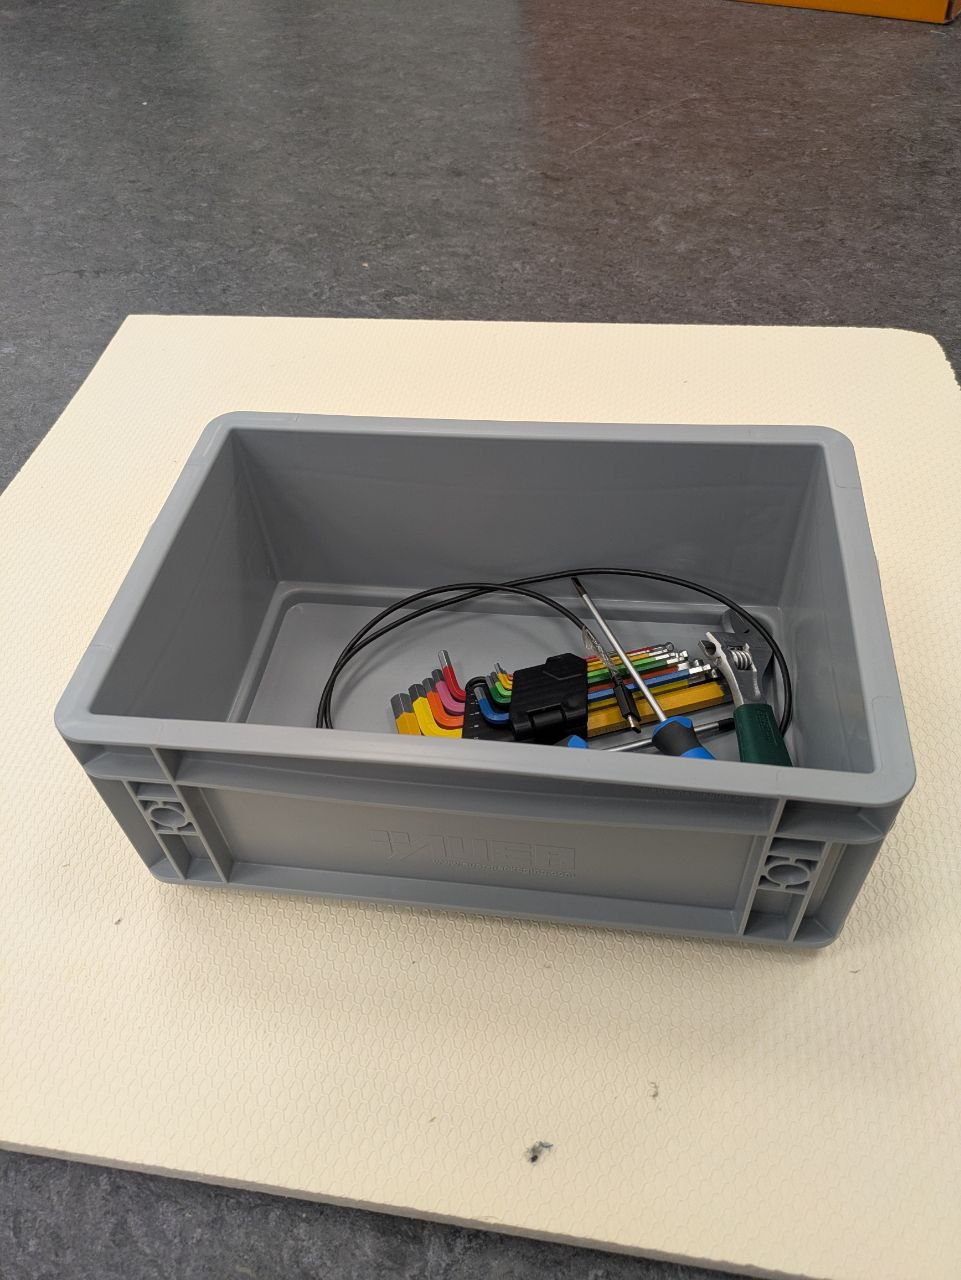
\includegraphics[trim=2cm 11cm 1cm 14.3cm, clip, width=0.6\linewidth]{images/eurobox.jpg}
    \caption{EG3212 Euro box that can serve as container for tools and materials.}
    \label{fig:box}
\end{figure}

Core research topics include planning and optimization under uncertainty, replanning and execution monitoring, fleet management, handling of dynamic events, and the integration of digital twins for prediction and monitoring.

% \subsubsection{Long-Term Vision}
The long-term objective is to enable comprehensive, factory-wide planning, diagnostics, and predictive capabilities across a heterogeneous set of entities, including robots, machines, and human workers. Coordination spans perception, planning, and execution, enabling continuous adaptation to uncertainty, dynamic events, and human intervention. Such coordination may also extend across multiple tracks.


% \subsubsection{Short-Term Focus}
% The short-term focus is planning transportation tasks for only intra-production logistics track robots. Teams
% perform planning and execution for predetermined product recipes without uncertainty, using Euro-Boxes.



\section{Transition from Former Industrial Leagues to SML}
\label{sec:transition}
%\todo[inline]{clarify that both leagues did something similar and how we solve this issue}
%\todo[inline]{mention the differences between them on a conceptional level is: packing boxes, transporting boxes, assembling box content}
\begin{tcolorbox}[disclaimerbox, title=Disclaimer]
This section is similar to \emph{Section 3 Task Description} of the reference proposal, which presents a more concrete initial scenario (\url{ https://github.com/robocup-at-work/sml-embodied-autonomous-intelligence}).
\end{tcolorbox}


The Smart Manufacturing League (SML) builds upon the achievements and philosophies of prior industrial leagues, extending their scope to better align with contemporary industrial requirements. Existing robotic platforms remain relevant, and the updated regulations are designed to preserve compatibility with prior constraints on a best-effort basis. While certain adaptations may be required, particularly regarding end-effectors and sensing systems, the anticipated financial impact on teams transitioning from previous competitions is limited.

To support diverse robotic system designs, the league standardizes workspace configurations into two main categories: ground-level, similar to the former @Work League, and human-operation height, similar to the former logistics league.

Conceptually, the former @Work and logistics leagues addressed similar challenges, primarily transporting objects around the shop floor. However, @Work emphasized short-term planning and complex manipulation, while the logistics league focused on intra-production logistics tasks requiring long-term planning. The SML accommodates both approaches by offering a Warehouse Track, which focuses on mobile manipulation with diverse objects, and an Intra-Production Logistics Track, which emphasizes planning and optimization using standardized Euro boxes to support a wide range of production scenarios. Teams are not required to enter a specific track; participation in any track is encouraged.

To ensure a smooth transition into the new formats, the initial manufacturing domain of the SML should be kept simple, allowing teams to focus on the shifting competition format and associated challenges.
One possible approach is the use of small interlocking toy bricks as base materials.
These can be sorted and placed into Euro boxes, transported to assembly stations, and combined into larger structures.

This scenario provides a suitable baseline for beginner-tier competitions or potential future Junior League formats, as it involves lightweight, simply shaped objects. Ultimately, the SML is not limited to a single domain.
Future challenges may incorporate a range of production scenarios, including industrial materials (e.g. screws, axles, soft materials) and assembly steps requiring tools (e.g. a screwdriver).




% The new league builds upon the achievements and philosophy of the former industrial leagues, broadening their scope to better align with current industrial requirements.

% Existing robotic platforms retain their relevance, and the revised regulations have been formulated to preserve compatibility with prior constraints. Although certain modifications, especially concerning end-effectors and sensing systems, may be necessary, the anticipated financial impact on teams of the former competitions should be limited.

% To accommodate different approaches of robotic systems, the workspace design for the robots is standardized in two categories: ground platforms (such as in the former @work league) and human operation height (such as in the former logistics league). They share the general shape and vary only in operating height and otherwise allow any viable solution for single- or multi-robot-systems. An example is depicted in Figure \ref{fig:table_height_graphic}.

% \todo[inline]{cite other concept paper}
% \todo[inline]{At Section 6.6 Arena Elements at @work'side concept paper. The size of EuroBox is "30 cm x 40 cm x 12 cm)" from @work vision. I think they assume the boxes are fixed (optionally bring out).}

% \begin{figure}[H]
%     \centering
%     \includegraphics[width=0.9\linewidth]{images/table_heights_3.png}
%     \caption{Tables (blue) on ground and human operating level for easy collaboration across different system designs, utilizing elevation platforms for static manipulators (purple).}
%     \label{fig:table_height_graphic}
% \end{figure}


% \subsection{Example Task Description}

% The SML represents a smart factory scenario where autonomous robots process product orders and returns on demand. %This setting encompasses multiple sub-tasks, such as operating assembly stations/workbenches, preparing and inspecting goods, recycling waste, managing intra-production logistics and dealing with uncertain events and disruptions.
% To account for the diversity of real-world industrial environments, the league employs a simplified scientific abstraction implemented as a competition framework that may change over time as the SML develops.

% The initial domain is based on small polymer building blocks (e.g. LEGO Duplo\texttrademark).
% Product designs can range from simple objects to multi-component goods, which may be unknown to teams prior the competition.
% A reference object set is displayed in Fig. \ref{fig:example_objects}. Future challenges will introduce more realistic industrial materials (e.g. screws, axis, soft materials) or add advanced assembly steps that require tools (e.g. a screwdriver).

% \todo[inline]{cite other concept paper}
% \todo[inline]{At Section 6.1 Objects and Materials at @work'side concept paper which is same as Section 5.1 of ours. They show the LEGO's image.}

% % \begin{figure}[H]
% %     \centering
% %     \includegraphics[width=0.8\linewidth]{images/example_mat_obj.png}
% %     \caption{Initial (basic) set of raw materials and objects used to perform assembly and recycling tasks in the new SML. These objects may change in future years, according to feedback from teams and learnings from upcoming events.}
% %     \label{fig:example_objects}
% % \end{figure}


\section{Competition Design and Scoring}
\label{s: competition_design}
The league is structured into track-specific competitions as well as a unified competition scenario that integrates the tasks of all tracks. While the track-specific competitions are initially likely conducted independently, the long-term vision is to run them concurrently on a shared field, forming a coherent smart factory environment.


Additionally, the option to branch into the RoboCup Junior competition will be explored.

\subsection{Track Competitions}
The goal of the SML is to provide a low entry barrier for beginner teams while still offering competitive benchmarks that challenge advanced researchers. To this end, each competition is structured into multiple tiers, ranging from introductory tasks for beginners to advanced problems targeting expert teams. Higher tiers correspond to increased task difficulty and yield higher scores.

There will be a best-in-track scoring system, where key performance metrics are defined separately for each track, allowing for fair comparison between teams within the same track to foster specialization competence in the defined areas.

\subsection{Unified Competition}

The unified competition promotes this convergence from the beginning by ensuring compatibility of tasks across tracks. At the same time, it provides room for generalized robotic solutions that might otherwise be disadvantaged when competing directly against highly specialized systems. The unified scenario further supports the use of heterogeneous robot fleets and explicitly encourages collaboration between teams participating in different tracks to jointly compete.

To ensure fairness, mechanisms will be introduced that allow single, general-purpose robots to compete effectively against coordinated multi-robot systems, for example through adaptive task allocation or adjusted scoring schemes. In addition, the unified competition may comprise a broad set of tasks spanning those defined in the individual tracks as well as supplementary tasks relevant to end-to-end industrial scenarios, such as machine inspection or cleanup operations.

Teams earn points based on the successful and timely completion of tasks, thereby incentivizing robots to handle a wide variety of tasks rather than optimizing for a narrow subset.

% Lastly, the competitions should foster a continuous production scenario, as required when performing 24/7 production, by establishing a slot system for each track. Teams may either book or get assigned to slots with the goal to continuously keep the factory running while teams change on-the-fly throughout a competition day.
% Unified solutions and track-specific robots should ultimately operate in the same arena at the same time under fair conditions, such that there is continuous action on the field.


\section{Technical Regulations}
\label{s: technical_regs}

The core idea of the SML is to allow almost any viable solution for used robotic systems. Teams are explicitly encouraged to come up with their unique designs and benchmark them in the new league to allow for a broader spectrum of evaluated solutions.

Teams are also allowed to use the same robot for multiple tracks. This allows using both a single, advanced robot (e.g. a humanoid), or a robotic fleet consisting of (multiple) specialized warehouse and workbench robots.

\subsection{Objects and Materials}
Industrial products can range from small nuts to complex devices, depending on the sector of each company.
However, the used materials and components often require specialized and often expensive hardware (e.g. strong manipulators) and largely vary in size, shape and weight. 

In order to allow teams to utilize low cost actuators while still retaining a large variety of materials and products, the SML focuses on standardized and lightweight materials that fit in Euro boxes of a defined size. 
These standardized containers are a globally available and cheap storage solution used in various industrial applications. The EG3212 box is the smallest available size ($300mm\times200mm\times120mm$) and offers a good compromise between handling and storage capacity for our competition scale.
However, the slightly bigger EG4312 spec ($400mm\times300mm\times170mm$) might also be a good option, if more space is needed.

\subsection{Robot Platforms}
To foster innovation and accommodate a wide range of technical approaches, the SML imposes minimal constraints on robot platform design across all tracks. Teams may deploy any type of robotic platform, including (but not limited to) wheeled robots, mobile manipulators, humanoids, or hybrid systems. No restrictions are imposed on the number of manipulators, tooling, or mechanical design.

All robots must operate fully autonomously and safely within the competition environment and must reliably interact with other robots, infrastructure, and human workers. To support factory-wide coordination, platforms are required to expose standardized interfaces for monitoring and control.

Robots with a footprint fitting within a 1 × 1 m cell and a mass that allows safe handling (carrying or pushing) by two people are permitted by default. Platforms exceeding these limits may be admitted upon prior approval by the organizers.

All computation hardware must be physically present at the competition site, either integrated into the robot or provided as dedicated off-field servers. The use of cloud-based computation is not permitted.

Robot motion capabilities must support throttling to competition-defined speed limits, as well as having an emergency stop. Unless otherwise specified, maximum actuator or platform speeds are expected to be on the order of 1.5 m/s.
\subsubsection{Warehouse Track Platforms}

Warehouse track robots must support autonomous logistics, mobile manipulation, and human-robot interaction across the production floor. Platforms are required to:
\begin{itemize}
    \item autonomously navigate shared shopfloor environments and avoid static and dynamic obstacles,
    \item perceive, locate, and inspect objects on storage infrastructure,
    \item pick up, transport, and deliver items, % to target stations,
    \item safely and predictably interact with human workers, including shared-space operation and implicit or explicit coordination with human actions.
\end{itemize}

%Teams may deploy a fleet of up to three robots.
Payload capacity, manipulation mechanisms, and fleet composition are otherwise unrestricted, enabling both single highly capable robots and collaborative multi-robot solutions. 
The payload of individual items to be lifted shall not exceed 1\,kg.

\subsubsection{Workbench Track Platforms}

Workbench track platforms focus on precise manipulation, assembly execution, and close-range human-robot interaction. Robots are required to:
\begin{itemize}
    \item accurately grasp, place, assemble, and disassemble objects,
    \item execute ordered task sequences with repeatable precision,
    \item collaborate safely with humans, for example through shared workspaces, handovers, or human-in-the-loop execution.
\end{itemize}

Teams may employ stationary systems, mobile robots, humanoids, or coordinated multi-manipulator setups. Multi-robot systems are permitted but optional, and may be used to distribute complementary capabilities or to trade individual robot complexity for coordinated operation. The payload of individual items to be lifted shall not exceed 1\,kg.

\subsubsection{Intra-Production Logistics Track Platforms}

Intra-Production Logistics platforms emphasize explicit fleet coordination, shopfloor optimization, and robust operation under uncertainty and disruptive events. Robots are required to:
\begin{itemize}
    \item autonomously navigate between production stations and buffers,
    \item transport standardized containers (Euro boxes),
    \item execute assigned transport tasks while reporting execution state,
    \item coordinate at the fleet level, including task allocation, scheduling, and conflict resolution,
    \item adapt plans in response to dynamic events, execution failures, and uncertainty.
    \item accept and integrate task requests from human operators, for example through explicit order submission or intervention at runtime.
\end{itemize}

%Teams may deploy a fleet of up to three mobile robots. 
As the focus of this track is fleet coordination, the use of a robot fleet is expected.
Using fewer robots, although allowed, may result in reduced competitiveness.
Platform design and locomotion are unrestricted, provided robots expose standardized interfaces to support centralized or distributed planning, execution monitoring, and replanning. The payload of carried containers shall not exceed 2\,kg.


\subsubsection{Unified Competition Platforms}
Robots in the unified competition need the skillset outlined in the individual tracks above.
Teams may deploy a robot fleet.% of up to three robots.
Scoring will be scaled based on the fleet size to make single-robot solutions feasible.

\subsection{Communication, Interfaces, and Data Traces}

The Smart Manufacturing League will define standardized communication interfaces and data formats for task allocation, coordination, and execution at the operational level.
Teams remain free to design and use any internal communication mechanisms or system architectures they deem appropriate.
However, when interacting with the shared shopfloor environment, teams are required to expose standardized interfaces and communicate explicitly with the league infrastructure to enable coordination, supervision, and logging.

Specifications will be developed in collaboration with competing teams to ensure minimal implementation overhead while supporting comprehensive monitoring, analysis, and benchmarking.
Established industrial standards, such as ISA-95~\citep{isa95} (along with its accompanying B2MML schemas ~\citep{b2mml}) and VDA~5050~\citep{vda5050}, will serve as a baseline to ensure that collected data traces and interfaces align with modern smart factory requirements.


The goal is to provide a data streaming and storage infrastructure that captures the relevant data and constitutes the backbone of league infrastructure, such as visualization for referees and the audience, referee systems that aid scoring and rule enforcement, and data analysis pipelines to support offline analysis, cross-team comparison, and long-term benchmarking of autonomous manufacturing systems.

Experience from the development and operation of the RefBox system~\citep{refbox16} in the RoboCup Logistics League provides several important insights for the design of the SML infrastructure.
First, it proved essential to maintain a central authority over shop-floor interactions in order to aggregate and synchronize heterogeneous data sources, including robots, machines, and referee inputs.
Second, the RCLL highlighted the critical importance of a well-designed data storage and access infrastructure.
While the RefBox enabled automated supervision and scoring, data persistence and structured access were only retrofitted at later stages, making post-hoc analysis cumbersome.
This limited the efficient extraction of higher-level representations, such as object-centric event logs (OCEL)~\citep{ocel21}, and the systematic capture of team intent and decision-making processes.
These lessons directly inform the SML vision, where data management is treated as a first-class design concern from the beginning.

\subsection{Arena}
All tracks share the same arena that acts as the factory floor.
% All competitions in the SML are played in a single shared arena that acts as the factory floor.
The arena will have similar total dimensions as the playing fields of the former leagues (at most in the order of $120m^2$).
All core elements of the arena will be designed to be easily obtainable so that there are now issues building arenas locally at competitions or in university labs.
The arena arena layout may evolve over the years, but initially, the arena will likely consist of boundary and corridor walls, storage shelves and workbenches and all elements should accommodate for both operation heights (see Section \ref{sec:transition}).

%\todo[inline]{cite other concept paper}
%\todo[inline]{At Section 6.7 Arena Layout at @work'side concept paper. Do we use the same figure or Till's figure?}
%\todo[inline]{We actually don't think @work'side concept paper or our old figure is a good solution. Therefore we would prefer to not show an image at all.}

% Figure \ref{fig:arena_dimensions} shows an example arena layout.
% \begin{figure}[h!]
%     \centering
%     \includegraphics[width=0.9\linewidth]{images/arena_dimensions_2.png}
%     \caption{Exemplary arena dimensions and layout. The design aims to create interesting planning and navigation scenarios, while keeping space requirements low. A mirrored layout with open doorways could allow for shared space operation of different team fleets, while closing them creates parallel performance scenarios without obstructions.}
%     \label{fig:arena_dimensions}
% \end{figure}


\section{Technical Challenges}
\label{sec:challenges}
\begin{tcolorbox}[disclaimerbox, title=Disclaimer]
This section is adopted from \emph{Section 10 Technical Challenges} of the reference proposal, where the section was jointly drafted (\url{ https://github.com/robocup-at-work/sml-embodied-autonomous-intelligence}).
\end{tcolorbox}
As part of the RCSML, we offer to host a set of technical challenges, which cover interesting problems that are not directly covered by any of the tracks. Unlike the tracks, which are a fixed part of the league, challenges are more dynamic and not permanent to the competition. They serve as a non-mandatory benchmark to test ideas and team performances for novel tasks that may be integrated into future track designs.
Each track may additionally host annual technical challenges addressing specific sub-problems such as tool use or environment exploration, allowing teams to experiment beyond standard competition tasks.
We explicitly encourage the community and the industry to approach the EC and TC with proposals.

Potential challenges include, but are not limited to:
\begin{description}[labelwidth=\widthof{\bfseries Industry-sponsored Challenges}]
    \item[Industry-sponsored challenges] We especially encourage industrial partners of the RCSML to post R\&D challenges, relevant to their production process, as part of the competition. % Integrating VDA5050 support will ease inclusion of hardware/software components developed in industry into these challenges.
    \item[Real-product challenges] Assembly tasks for real products including realistic components of different materials. One typical example could be a drive train consisting of gear boxes, drive shafts and actuators. 
    \item[Anomaly-detection challenges] Robots might be required to detect and report unexpected situations, such as faulty materials, unsorted shelves or broken tools, with the goal of autonomously resolving such situations.
    \item[Simulation challenges] Simulation environments for workbench and/or Intra-Production Logistics track tasks are developed which allow for simulated competitions.
\end{description}


\section{Comparison to \texorpdfstring{\emph{Embodied Autonomous Intelligence for \\ On-Demand Manufacturing: A RoboCup Industrial Workshop Proposal}}{Embodied Autonomous Intelligence for On-Demand Manufacturing: A RoboCup Industrial Workshop Proposal}}

We would also like to explicitly discuss the relationship between this concept paper and the reference proposal
\emph{Embodied Autonomous Intelligence for On-Demand
Manufacturing: A RoboCup Industrial Workshop Proposal}.

In the following, we outline the similarities and differences between the two approaches.

On the one hand, both papers agree that the challenges of modern smart manufacturing should be tackled through different tracks and also including beginner friendly difficulty tiers. Technical regulations should be open, such that all robotic platforms are welcome and that as a first scenario, a production facility utilizing interlocking toy bricks sounds like a promising start.

Our paper does deliberately not cover specifics, such as arena layouts, concrete tasks for the first competition and scoring schemes, as we believe these should follow only after settling on a conceptual foundation.

However, core differences arise in the following areas:
\begin{itemize}
\item \textbf{Intra-logistics and Planning Design}
In the reference proposal, intra-logistics operations are incorporated into the warehouse track without relying on standardized containers for transport, using them only for storage. Long-term planning is addressed separately in a dedicated simulation-based planning track, which evaluates task-level strategies using a 2D simulation similar to the RCLL simulator\footnote{\url{https://github.com/robocup-logistics/rcll-simulator}}.  

We argue that long-term planning should be tightly coupled with physical interaction. Our experience in the Logistics League repeatedly showed that purely simulation-based plan execution suffers from the sim-to-real gap and cannot replace real-world benchmarking. In industrial applications, intra-production logistics is critical. While manipulating standardized boxes or pallets is largely a solved problem, the real challenge lies in fleet coordination, plan optimization, and robustness under uncertain events and perturbations.  

The RCLL demonstrated the value of this approach within a constrained factory setup (Festo MPS).
We believe that extending this principle to more heterogeneous environments with additional operational challenges will significantly increase both scientific relevance and industrial applicability.

In the SML, we propose a dedicated Intra-Production Logistics track, rather than relying on warehouse robots to handle these tasks. This separation makes it feasible to evaluate long-term planning in a physical competition without being frequently disrupted by complex manipulation failures.
At the same time, sophisticated mobile manipulation can still be explored in a separate track.

While it would also be possible to integrate intra-logistics planning into the warehouse track, we argue that both intra-logistics planning and general mobile manipulation are substantial enough areas to justify separate tracks.
This approach allows teams to demonstrate advanced planning and coordination capabilities without requiring a diverse mobile manipulation skill set, ensuring that each core competency can be meaningfully assessed.
\item \textbf{Competition Design and Scoring}

In the reference Workshop Proposal, scores from all tracks are combined into a single cumulative result. This design encourages participation across all tracks and fosters long-term collaboration between teams, emphasizing collective engagement rather than specialization. 

In contrast, the SML concept implements a best-in-class scoring system, recognizing team performance within specialized tracks and enabling track-specific metrics that capture the unique challenges of each domain without forcing a comparison across fundamentally different tasks. Simultaneously, a unified factory challenge evaluates generalization, rewarding systems that can successfully tackle multiple tracks at once. This dual structure encourages both deep expertise in individual areas and the development of versatile, all-rounder robotic solutions.  

Beyond scoring, the expert tracks are designed to operate within a single integrated production scenario. Competitions for each track are intended to be hosted simultaneously on the same field, allowing the tracks to interact organically.

% TODO: long-term vision and industrial relevance: is actually quite close due to our points being present in that paper aswell

\item \textbf{Human–Robot Interaction (HRI)}

The reference Workshop Proposal explicitly acknowledges human–robot interaction as a relevant aspect of embodied autonomous intelligence, for example by highlighting interaction with humans or other machines and coordination across multiple agents.
However, these aspects are discussed at a high level and remain largely conceptual.
Human involvement is primarily framed as an enabling mechanism to compensate for missing autonomous capabilities or to keep the overall factory scenario operational, rather than as a central driver of task design.

In contrast, the SML concept treats human–robot interaction as a first-class research challenge and explicitly integrates it into the design of individual tracks.
HRI is operationalized through concrete interaction scenarios, emphasizing safe, structured, and meaningful collaboration in shared workspaces.
This includes, for example, task handovers, interaction-aware planning, coordination under human presence, and controlled human intervention.
By embedding HRI directly into competition tasks and benchmarks, we position human–robot interaction as a core research problem that remains largely unsolved in modern industrial settings and demands thorough and systematic study.

\item \textbf{Communication Infrastructure and Data Management}

The reference Workshop Proposal does only briefly mention the need for standardized league-wide communication.

In contrast, our concept treats communication and data management as a core element of the league. Standardized interfaces are mandatory for interaction with the shopfloor and league infrastructure, enabling coordinated execution, reproducible evaluation, and comprehensive logging across heterogeneous robotic systems.
\end{itemize}
\section{Open Discussion}
This document focuses primarily on the long-term direction of the Smart Manufacturing League, aiming to ensure relevance for research and industry for years to come.
At this stage, it incorporates insights from past interactions from RoboCup events and with industrial partners but does not yet include targeted feedback from the broader community.  

Many core design points (such as concrete arena constraints, scoring schemes or limitations on fleet sizes) remain intentionally open for discussion.
We encourage teams, committee members, and other stakeholders to contribute their perspectives, particularly on aspects where no consensus or definitive guideline exists. Key open points include:

\begin{itemize}
    \item \textbf{Initial Track Scope:} Which core problems should be tackled in the initial competition for each track? Is the track selection sufficient or are more/different tracks needed?
    \item \textbf{Initial Production Scenario}: What are the core tasks that we want to establish for the first full competition?
    \item \textbf{Robot fleet sizes:} What is the constraints and target number of robots in warehouse, intra-production logistic and the unified track? Are constraints or targets on the number of end-effectors necessary in the workbench and assembly track?
    \item \textbf{Workstation and table heights:} Should the league be open to continue with both human-operation and ground-floor level tasks? If yes, how can we ensure a smooth competition with minimal effort to accommodate for both? If no, how can we transition to a uniform solution without discouraging teams that have to adapt accordingly?
    \item \textbf{Container Dimensions}: What is the most suitable Euro box size for use in the SML?
    \item \textbf{Inspection tasks:} Should inspection be integrated into existing tracks, or treated as a separate future track?
    
    \item \textbf{24/7 competition suitability:} How can the league design accommodate continuous operation scenarios?
    
\end{itemize}

Community feedback is welcome and will be used to iteratively refine this document regarding regulations, track designs, and scoring mechanisms, ensuring that this concept paper can provide a vision of the SML that remains both scientifically challenging and broadly accessible.

%\todo[inline]{discussion points which should be addressed where we have no hard opinion like:}
%\todo[inline]{inspection as part of other tracks or a future one}
%\todo[inline]{table height as a long-term goal}
%\todo[inline]{additional tasks for workshop track and unified competition}
%\todo[inline]{24/7 competition suitability}



\FloatBarrier
% =================================================

% \newpage

% \vfill

\bibliographystyle{plainnat}
\bibliography{references}

\end{document}
